\documentclass[notes]{beamer} 
%\usepackage{pgfpages}
%\setbeameroption{show notes on second screen=right}
\usepackage[british]{babel}
\usepackage{graphicx,hyperref,ru,url}
\usepackage{listings}
\usepackage{xcolor}

\definecolor{red}{RGB}{190,49,26}
\title[Model-Based Testing]{Model-Based Testing}
\subtitle{An overview of existing tools}

%\author[Pedro Tavares \& Raquel Dias]{
%    \parbox[t][][t]{2in}{Pedro Tavares \\ \texttt{up201708899@fe.up.pt}}
%    \and 
%    \parbox[t]{1.5in}{Raquel Dias \\ \and \texttt{up201700419@fe.up.pt}}
%}

\author[Pedro Tavares \& Raquel Dias]{%
  \texorpdfstring{%
    \begin{columns}
      \column{.4\linewidth}
      \centering
      Pedro Tavares \\ \texttt{up201708899@fe.up.pt}
      \column{.4\linewidth}
      \centering
      Raquel Dias \\ \texttt{up201700419@fe.up.pt}
    \end{columns}
 }
 {Pedro Tavares, Raquel Dias}
}

\institute[Faculty of Engineering of the University of Porto]{Faculty of Engineering of the University of Porto}

\date[MESW1718-TVVS]{MESW1718-TVVS \\ 15 December 2017}

\begin{document}

\begin{frame}
  \titlepage
\end{frame}

\section{Introduction}

\begin{frame}
  \frametitle{Model-Based Testing}
  \setbeamercovered{transparent}
  \begin{definition}[Model-Based Testing]<1->
  Is a software \textbf{testing technique} that uses test generation algorithms and a behavioral model of the system under test to \textbf{generate test cases}.
  \end{definition}
  \begin{block}{}<2->
  It depends on three key technologies: the \textbf{notation} used for the data model, the test-generation \textbf{algorithm}, and the \textbf{tools} that generate supporting infrastructure for the tests.
  \end{block}
  \begin{block}{}<3->
  Instead of writing hundreds of test cases, the test designer writes an \textbf{abstract model} of the system under test, and then, the model-based testing tool \textbf{generates a set of test cases} from that same model.
  \end{block}
\end{frame}

\section{Tools Overview}

\begin{frame}
  \frametitle{Tools Overview}
  We'll take a look on the following tools:
  
  \begin{itemize}
  \item ModelJUnit
  \item Spec Explorer
  \item Graphwalker
  \item MISTA
  \end{itemize}
\end{frame}

\begin{frame}
  \frametitle{ModelJUnit}
  \setbeamercovered{transparent}
  \begin{itemize}[<+->]
    \item Extends from JUnit for model-based testing.
    \item Analyze a finite state machine written in Java and convert it into a corresponding visual representation.
    \item After the finite state graph is created, test cases can be automatically generated, customized, and executed based on user preferences.
    \item It was created by Dr. Mark Utting, but it seems to be abandoned.
  \end{itemize}
  
\end{frame}

\begin{frame}[fragile]
\frametitle{ModelJUnit}
\framesubtitle{Finite State Machine}

\begin{figure}
\centering
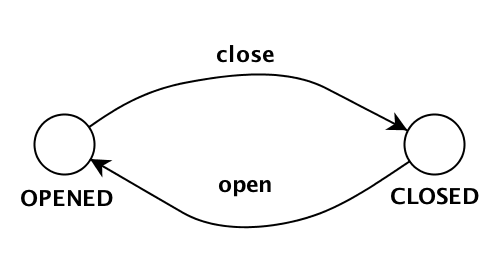
\includegraphics[scale=0.8]{finite-state-machine.png}
\caption{Simple Finite State Machine with two possible states: \texttt{Opened} and \texttt{Closed} and two events: \texttt{open}, that shifts from state \texttt{Closed} to \texttt{Open}; and \texttt{close}, that shifts from state \texttt{Open} to \texttt{Closed}.}
\label{fig:finite-state-machine}
\end{figure}
\end{frame}

\begin{frame}[fragile]
\frametitle{ModelJUnit}
\framesubtitle{Implementation}
\begin{lstlisting}[language=Java,basicstyle=\ttfamily,keywordstyle=\color{red},caption={Snippet that represents a transition/event of the model. It must use the \texttt{@Action} annotation. Guards can also be defined. In this case, it can only move to closed if the current state is open.}, captionpos=b]
public boolean Move_To_Closed_Guard() {
  return this.state == State.OPEN;
}

@Action public void Move_To_Closed() {
  this.state = State.CLOSED;
}

\end{lstlisting}
\end{frame}

\begin{frame}
  \frametitle{Spec Explorer}
  \setbeamercovered{transparent}
  \begin{itemize}[<+->]
    \item Allow to model applications using C\# and to generate state machine diagrams and unit tests from those models.
    \item It automatically generates test cases from very simple code that represents the model of the application.
    \item The generated test cases can be run against the implementation class, or they can be exported and run against the actual application.
    \item Documentation is available online on MSDN, as well as a couple of tutorials/examples.
  \end{itemize}
\end{frame}

\begin{frame}[fragile]
\frametitle{Spec Explorer}
\framesubtitle{Implementation}
\begin{lstlisting}[language=Java,basicstyle=\ttfamily,keywordstyle=\color{red},caption={Snippet that represents a transition/event of the model. It must use the \texttt{Rule} attribute. Guards are implemented in the same method.}, captionpos=b]
[Rule]
public static void Move_To_Closed() {
  Condition.IsTrue(this.state == State.OPENED);
  this.state = State.CLOSED;
}
\end{lstlisting}
\end{frame}

\begin{frame}
    \frametitle{Graphwalker}
    \setbeamercovered{transparent}
    \begin{itemize}[<+->]
        \item It generates test sequences from state machines modeled in GraphML with an external tool: yEd.
        \item It is designed to integrate with Java and Maven.
        \item Generate tests that can be run using a test tool like JUnit or Selenium.
        \item Each run generates a random run through the program that follow a path until reach all of the edges.
        \item Simple to acquire, hard to setup and customize.
    \end{itemize}
\end{frame}

\section{Selected Tool: MISTA}

\begin{frame}
  \frametitle{MISTA}
    \setbeamercovered{transparent}
    \begin{itemize}[<+->]
    \item It uses lightweight high-level Petri Nets as a visual modelling notation.
    \item It generates executable test code from a test model to several languages and testing frameworks. (Java and JUnit included)
    \item It make sure that all states and transitions in a model can be reached.
    \item Models can be built either using a GUI interface or a spreadsheet editor.
    \item Well suited for test-driven development.
    \item Simple to acquire. It is just a simple Java JAR application.
  \end{itemize}
\end{frame}

\begin{frame}
  \vspace{-20.5pt}
  \frametitle{MISTA}
  \vspace{-20.5pt}
  \framesubtitle{Petri Nets}
  \begin{figure}
    \centering
    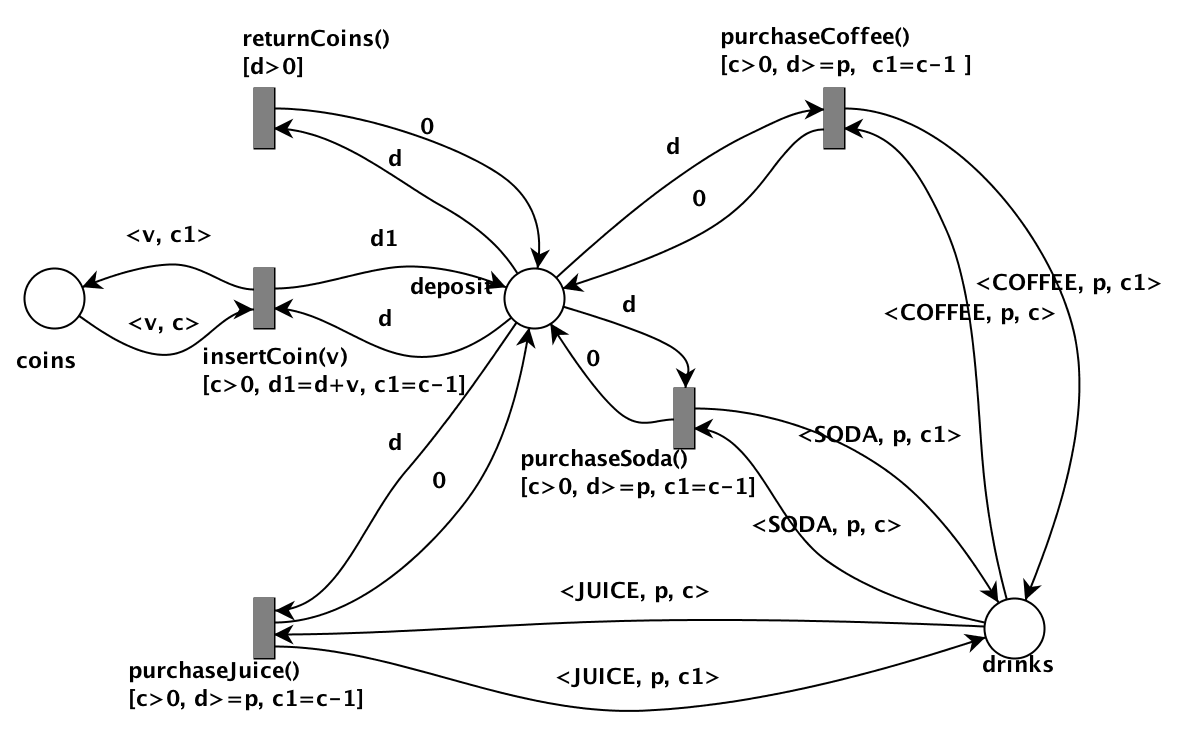
\includegraphics[scale=0.4]{petri-net.png}
    \caption{Petri Net that represents a vending machine system.}
    \label{fig:finite-state-machine}
  \end{figure}
\end{frame}

\begin{frame}
  \frametitle{MISTA}
  \framesubtitle{Petri Nets}
  \setbeamercovered{transparent}
  \begin{definition}[Petri Net]<1->
    A Petri net consists of \textbf{places}, \textbf{transitions}, and \textbf{arcs}. Arcs run from a place to a transition or vice versa, never between places or between transitions.
  \end{definition}
  \begin{block}{}<2->
    The places from which an \textbf{arc runs to a transition} are called the \textbf{input} places of the transition.
  \end{block}
  \begin{block}{}<3->
  The places to which \textbf{arcs run from a transition} are called the \textbf{output} places of the transition.
  \end{block}
\end{frame}

\begin{frame}
  \vspace{-20.5pt}
  \frametitle{MISTA}
  \vspace{-20.5pt}
  \framesubtitle{Petri Nets}
  \begin{figure}
    \centering
    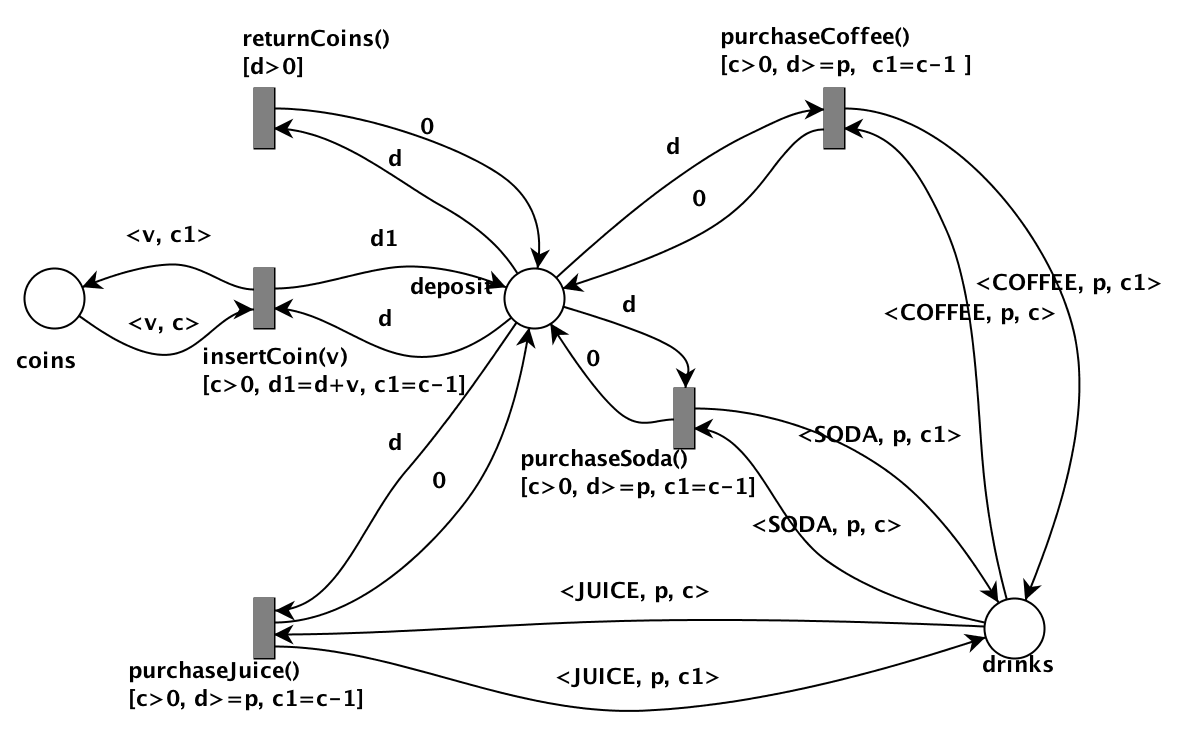
\includegraphics[scale=0.4]{petri-net.png}
    \caption{Petri Net that represents a vending machine system.}
    \label{fig:finite-state-machine}
  \end{figure}
\end{frame}

\begin{frame}
    \frametitle{MISTA}
    \framesubtitle{Petri Nets}
    \begin{columns}[t]
    \column{0.5\textwidth}
    The Vending System Petri Net has the following places:
    \begin{itemize}
        \item \texttt{coins}
        \item \texttt{deposit}
        \item \texttt{drinks}
    \end{itemize}
    \column{0.5\textwidth}
    The Vending System Petri Net has the following transitions:
    \begin{itemize}
        \item \texttt{insertCoin(v)}
        \item \texttt{returnCoins()}
        \item \texttt{purchaseJuice()}
        \item \texttt{purchaseSoda()}
        \item \texttt{purchaseCoffee()}
    \end{itemize}
    \end{columns}
\end{frame}

\begin{frame}
  \frametitle{MISTA}
  \framesubtitle{Some of the test coverage criteria available}
  \begin{itemize}
    \item \textbf{Reachability tree coverage}: generates the reachability graph with respect to all given initial states and, for each leaf node, creates a test from the corresponding initial state node to the leaf.
    \item \textbf{Transition coverage}: tests are generated to cover each transition.
    \item \textbf{State coverage}: tests are generated to cover each state that is reachable from any given initial state.
    \item \textbf{Depth coverage}: only the tests whose lengths are no greater than the given depth are generated.
  \end{itemize}
\end{frame}

\begin{frame}[fragile]
\frametitle{MISTA}
\framesubtitle{Example of a generated test}
\begin{lstlisting}[language=Java,basicstyle=\ttfamily,keywordstyle=\color{red},caption={Example of a generated test based on Reachability tree coverage. Tries to check if the vending machine deposit is empty after returning the coins.}, captionpos=b]
public void test116() throws Exception {
  System.out.println("Test case 116");
  vm.insertCoin(Coin.DOLLAR);
  vm.insertCoin(Coin.NICKEL);
  vm.purchase(COFFEE);
  vm.insertCoin(Coin.QUARTER);
  vm.returnCoins();
  assertTrue("1_1_1", vm.getDeposit() == 0);
}
\end{lstlisting}
\end{frame}

\begin{frame}
  \titlepage
\end{frame}

\end{document}
